\begin{figure}[H]
\centering
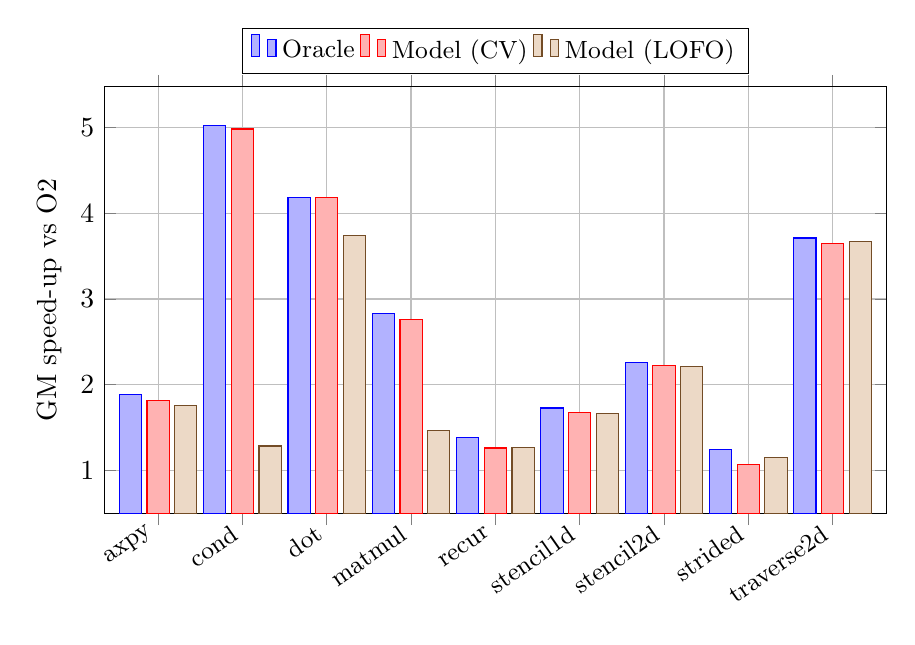
\begin{tikzpicture}
\begin{axis}[
    ybar, width=0.95\textwidth, height=7cm,
    ylabel={GM speed-up vs O2},
    symbolic x coords={axpy,cond,dot,matmul,recur,stencil1d,stencil2d,strided,traverse2d},
    xtick=data, x tick label style={rotate=35,anchor=east,font=\small},
    ymin=0.5, 
    bar width=8pt,
    enlarge x limits=0.08,
    legend style={at={(0.5,1.03)},anchor=south,legend columns=-1,font=\small},
    grid=major]
\addplot coordinates {(axpy,1.8813) (cond,5.0214) (dot,4.1862) (matmul,2.8279) (recur,1.3805) (stencil1d,1.7286) (stencil2d,2.2584) (strided,1.2434) (traverse2d,3.7099)};
\addplot coordinates {(axpy,1.8198) (cond,4.9817) (dot,4.1854) (matmul,2.7556) (recur,1.2621) (stencil1d,1.6731) (stencil2d,2.2253) (strided,1.0687) (traverse2d,3.6507)};
\addplot coordinates {(axpy,1.7556) (cond,1.2858) (dot,3.7438) (matmul,1.4649) (recur,1.2704) (stencil1d,1.6671) (stencil2d,2.2138) (strided,1.1561) (traverse2d,3.6741)};
\legend{Oracle,Model (CV),Model (LOFO)}
\end{axis}
\end{tikzpicture}
\caption{Per-family speed-up over \texttt{O2} for the k-NN: oracle, random-split cross validation, and leave-one-family-out.}
\label{fig:family}
\end{figure}
